\section{The \textit{SAE J2522} regulation}\label{the-sae-j2522-regulation}

		More related to this project is the \textit{SAE J2522}, entitled \textit{Dynamometer Global Brake Effectiveness}, at the beggining it already states the it's utility with the following:

		\say{The SAE Brake Dynamometer Test Code Standards Committee considers this standar useful in supporting the technological efforts intended to improve motor vehicle braking systems overall performance and safety}

		This regulation \cite{saej2522} was developed to be used in conjecture with other test standards in other to address the friction of a certain material to check it's adequacy for a certain application. It is important to mention that this work is based on the \textit{SAE J2522}, it is not a faithful application of the standard though. This paper is more concerned about the settings of the tests mentioned on the regulation rather than the formulas and criteria for a materials engineering analysis.
		\par
		All the tests mentioned on the regulation can generalised on repetitive cycles of accelerating the rotor to a specified speed and appling brake force (may vary along the test) until the rotor reaches a lower limit of speed. On the regulation, sometimes the desacceleration ratio is also defined but not always. Initial temperature is also defined, some tests can only be perfomed if the brake parts are under a certain temperature.

		\subsection{Monitored Parameters}\label{ssec:monitored-parameters}
			According to Regulation \textit{SAE J2522} \cite{saej2522}, in order to perform the brake tests specified it is mandatory to evaluate the following parameters:

			\begin{itemize}
				\item \textit{Temperature of the brake pads:} It is important during the entire test to be fully aware of the temperature of the brake system, firstly by the safety factor (there is a maximum operating temperature for the system), also by the wear of the system that is tied to the temperature therein. Last but not least is the fact that knowing the temperature it is possible to carry out tests based on it, being possible to make tests in known temperature ranges.\label{itm:monitored-temperature}
				\item \textit{Braking force:} The pressure to be measured is the pressure that the brake caliper is applying to the rotor over time, knowing the magnitude of this force means having control over how much the temperature increases according to braking and how much the rotor speed decreases as a function of braking.\label{itm:monitored-pressure}
				\item \textit{Rotation Speed:} Without knowledge of rotor speed it would be impossible to determine whether the brake is being effective or how effective it is. Speed monitoring is the most critical parameter for system operation, without it there is no utility to the rest of the equipment. \label{itm:monitored-speed}
			\end{itemize}

			Another interesting parameter to monitor that is not specified on Regulation \textit{SAE J2522} is the vibration on the caliper, usually when the magnitude of this vibration is considerably high it usually indicates that this part is already worn out \cite{goodyear-calipers} and it may damage the rotor by bending it over time. Is is also relevant to mention that vibration is measured in terms of \textit{g} (9.8 $m\cdot s^2$).

		\subsection{Brake Tests}\label{ssec:brake-tests}
			All tests specified on the regulation follow a certain pattern of execution order which is synthesized in Figure \ref{fig:brake-test-diagram}.

			\begin{figure}[htbp]
				\centering
				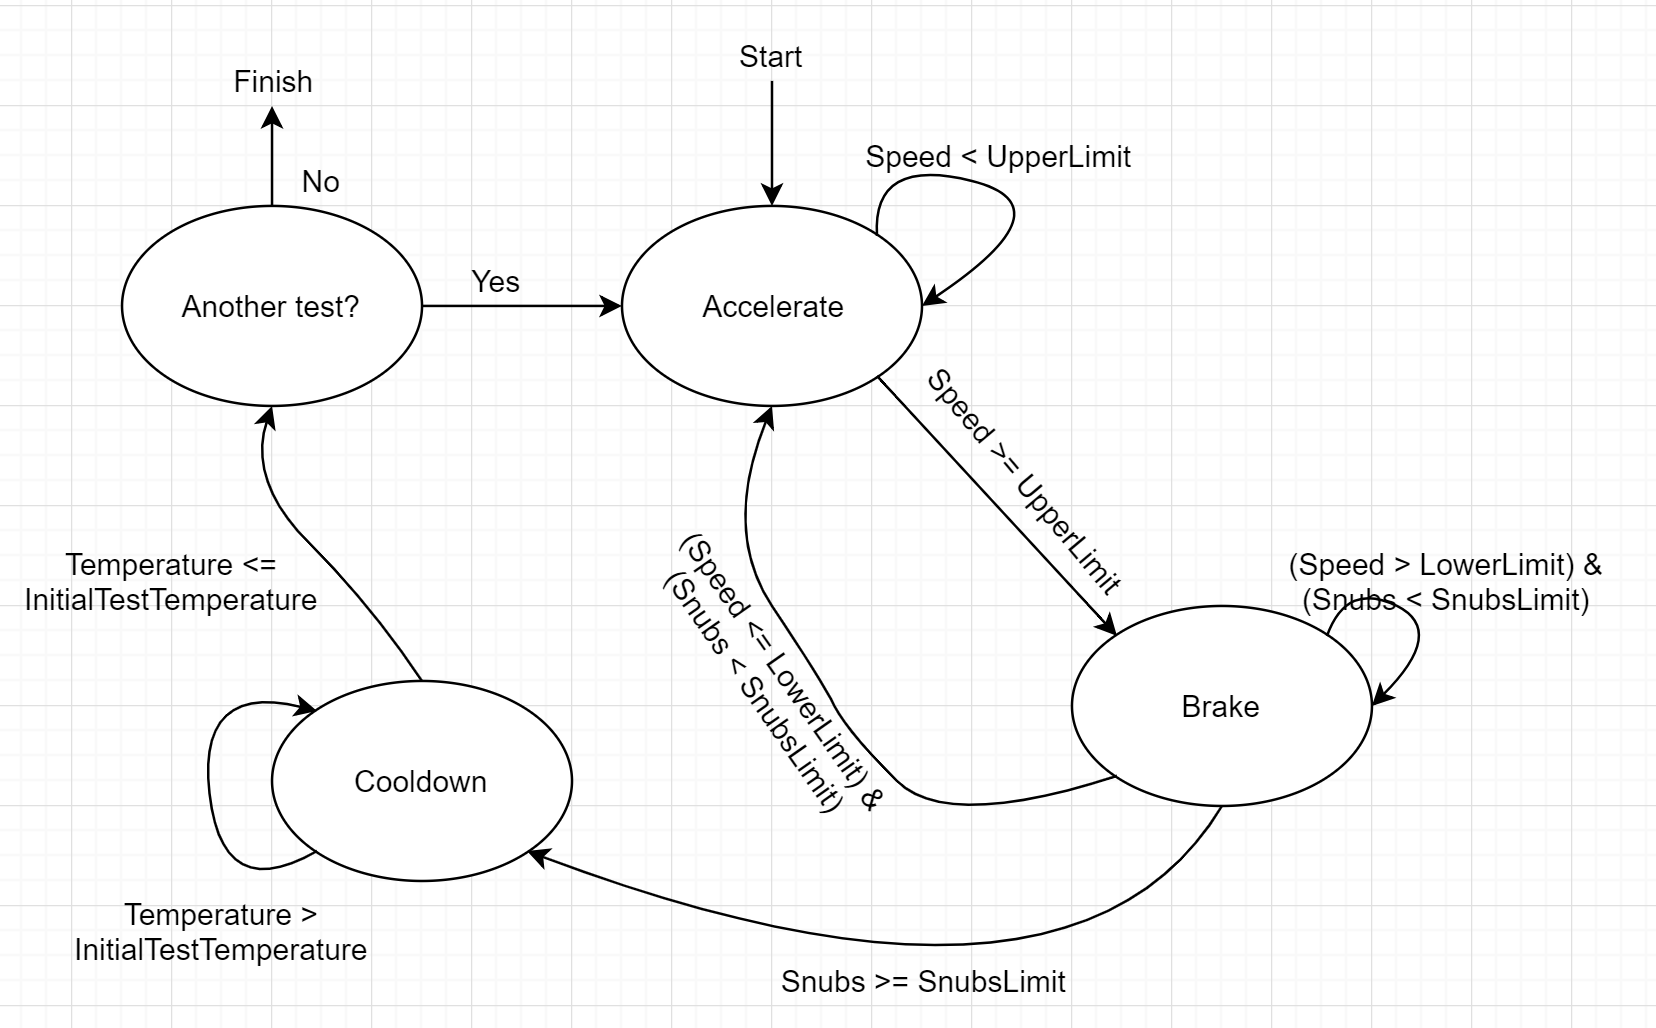
\includegraphics[width=.8\textwidth]{figuras/fig-brake-test-diagram}
				\caption{Brake Tests Diagram of Execution}
				\label{fig:brake-test-diagram}
			\end{figure}

			The system is accelerated to a top speed \textit{\textbf{(Upper Speed Limit)}}, than the brake actuates with a known force \textit{\textbf{(Brake Force)}} until the system reaches a certain speed \textit{\textbf{(Lower Speed Limit)}}, this process is repeated for certain number of times \textit{\textbf{(Snubs)}} and after each test the system must rest \textit{\textbf{(Cooldown)}} until the brakes are cooled enough regarding a defined cooldown time.